\documentclass[10pt,openright,twoside,french]{book}
\input philippe2013
\input philippe2013_activites
\pagestyle{empty}


\begin{document}

\TitreActivite{ii.2}{Fonction valeur absolue}

On appelle \textbf{valeur absolue} d'un nombre réel $x$ le nombre \textbf{positif}, noté $\abs x$, défini par :
\[\abs x =
\left\{\begin{array}{r@{ \text{ si } }l}
	x & x \geq 0 \\
	-x & x \leq 0
\end{array}\right.\]

\begin{enumerate}
	\item À combien est égale $\abs{12}$ ? Et $\abs{-12}$ ?
	\item Compléter le tableau suivant :\medskip

{
	\footnotesize
		\renewcommand{\arraystretch}{1.5}
		\begin{tabular}{|c|*{13}{>{\scriptsize\centering\arraybackslash}m{0.65cm}|}}
			\hline
				$x$ & $-3$ & $-2,5$ & $-2$ & $-1,5$ & $-1$ & $-0,5$ & $0$ & $0,5$ & $1$ & $1,5$ & $2$ & $2,5$ & $3$ \\
			\hline
				$\abs x$ &&&&&&&&&&&&& \\
			\hline
		\end{tabular}
}\medskip

\item Sur le repère ci-dessous, représenter la fonction $v \colon x \mapsto \abs x$.

\begin{center}
    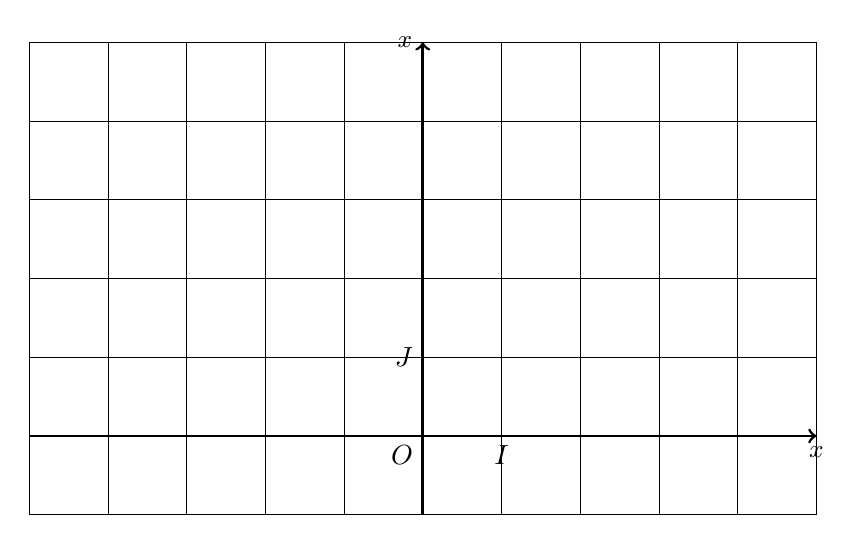
\begin{tikzpicture}[x=1cm,y=1cm]
        \draw[line width = 0.2pt] (-5,-1) grid[xstep=1,ystep=1] (5,5);
        \draw[line width = 1pt,->] (-5,0) -- (5,0) node[below] {\small $x$};
        \draw[line width = 1pt,->] (0,-1) -- (0,5) node [left] {\small $\abs x$};
        \coordinate (O) at (0,0); \draw (O) node[below left] {$O$};
        \coordinate (I) at (1,0); \draw (I) node[below] {$I$};
        \coordinate (J) at (0,1); \draw (J) node[left] {$J$};
    \end{tikzpicture}
\end{center}

\item Dessiner le tableau de variation de la fonction $v$ puis déterminer le minimum de $v$.
\item Sur l'intervalle $\intervalleof{-\infty}{0}$, la fonction $v$ coïncide avec quelle autre fonction ?
\item Même question sur l'intervalle $\intervallefo{0}{+\infty}$.
\end{enumerate}

\end{document} 